%%%%%%%%%%%%%%%%%%%%%%%%%%%%%%%%%
%
%       EXERCÍCIO
%
%%%%%%%%%%%%%%%%%%%%%%%%%%%%%%%%%

\ifdefstring{\atividade}{prova}{%
    \ifdefstring{\modo}{objetivo}{%
        \renewcommand{\valorquestao}{\ValorQObj\ ponto}
    }{%
        \renewcommand{\valorquestao}{\ValorQDisc\ pontos}
    }%
}%

\begin{exercicioBanco}[\valorquestao]
No diagrama a seguir, \(A\), \(B\) e \(C\) são três conjuntos não vazios.

\begin{center}
    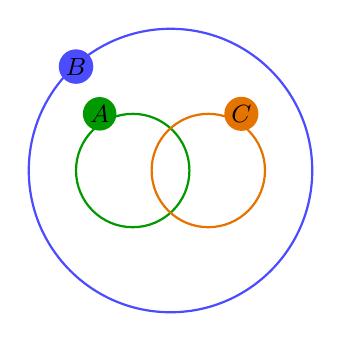
\begin{tikzpicture}[scale=0.6]
        % Conjunto B (maior)
        \draw[thick, blue!70] (0,0) circle (3);

        % Conjunto A (intersectando C)
        \draw[thick, green!60!black] (-0.8,0) circle (1.2);

        % Conjunto C (intersectando A)
        \draw[thick, orange!90!black] (0.8,0) circle (1.2);

        % Rótulos
        \node[circle, fill=blue!70, inner sep=1pt] at (-2,2.2) {\small$B$};
        \node[circle, fill=green!60!black, inner sep=1pt] at (-1.5,1.2) {\small$A$};
        \node[circle, fill=orange!90!black, inner sep=1pt] at (1.5,1.2) {\small$C$};
    \end{tikzpicture}
\end{center}

Assinale verdadeira (V) ou falsa (F) a cada uma das seguintes sentenças.

\begin{enumerate}[I.]
    \begin{multicols}{5}
        \item \(A \subseteq B\).
        \item \(C \subseteq B\).
        \item \(A \cap C = \varnothing\).
        \item \(A \cap C \subseteq B\).
        \item \(A \cup C = B\).
    \end{multicols}
\end{enumerate}

% Define as alternativas
\newcommand{\alternativas}{%
    \begin{center}
        \begin{tabularx}{\textwidth}{XXXXX}
            (a) (V, V, F, V, F). &
            (b) (V, V, V, F, F). &
            (c) (F, V, F, V, V). &
            (d) (V, F, F, V, F). &
            (e) (V, V, F, F, V).
        \end{tabularx}
    \end{center}
}

% Define a resposta correta
\newcommand{\resposta}{A}

% Lógica condicional para exibição
\ifdefstring{\atividade}{lista}{%
    \alternativas
    \vspace{0.5em}
    
    \noindent\textbf{Resposta:} letra \textbf{\resposta}.
}{%
    \ifdefstring{\modo}{objetivo}{%
        \alternativas
    }{%
        % modo = discursiva → não mostra alternativas
    }
}
\end{exercicioBanco}

